\begin{table}[H]
\centering
\begin{tabular}{| l | l | l |}
\hline
Type & RMSD & Percent \\ \hline
Under & 42 & 53.2\% \\ \hline
Over & 48 & 46.8\% \\ \hline
Total & 45 & \\ \hline
\end{tabular}
\caption{Exponential smoothing predictor results for the baseline workload}
\end{table}

\begin{figure}[H]
\centering
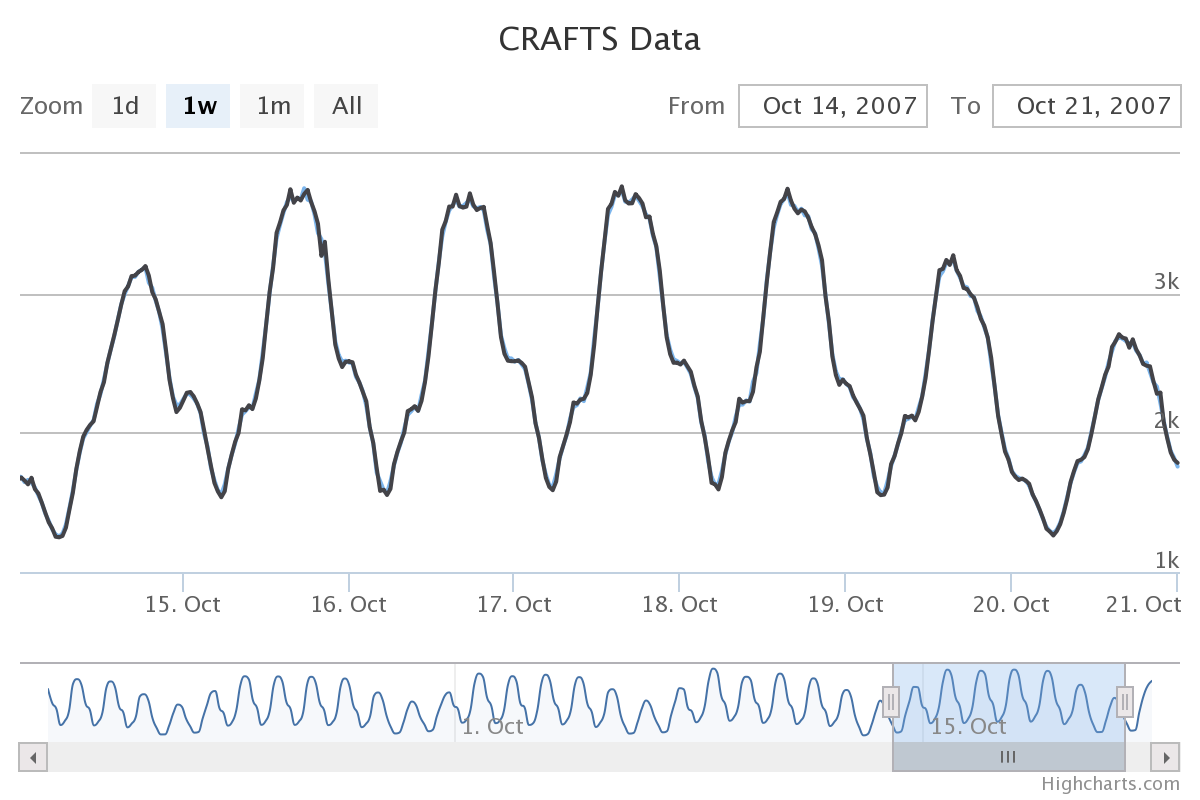
\includegraphics[width=\textwidth]{results/graphs/smoothing_baseline.png}
\caption{Exponential smoothing prediction results for the baseline workload}
\label{fig:smoothing_b}
\end{figure}

\begin{table}[H]
\centering
\begin{tabular}{| l | l | l | l | l |}
\hline
Type & \multicolumn{2}{c |}{Regular} & \multicolumn{2}{c |}{Anomalous} \\ \hline
 & RMSD & Percent & RMSD & Percent \\ \hline
Under & 42 & 53.1\% & 31 & 72.7\% \\ \hline
Over & 48 & 46.9\% & 22 & 27.3\% \\ \hline
Total & 45 & & 29 & \\ \hline
\end{tabular}
\caption{Exponential smoothing predictor results for the training outage workload}
\end{table}

\begin{figure}[H]
\centering
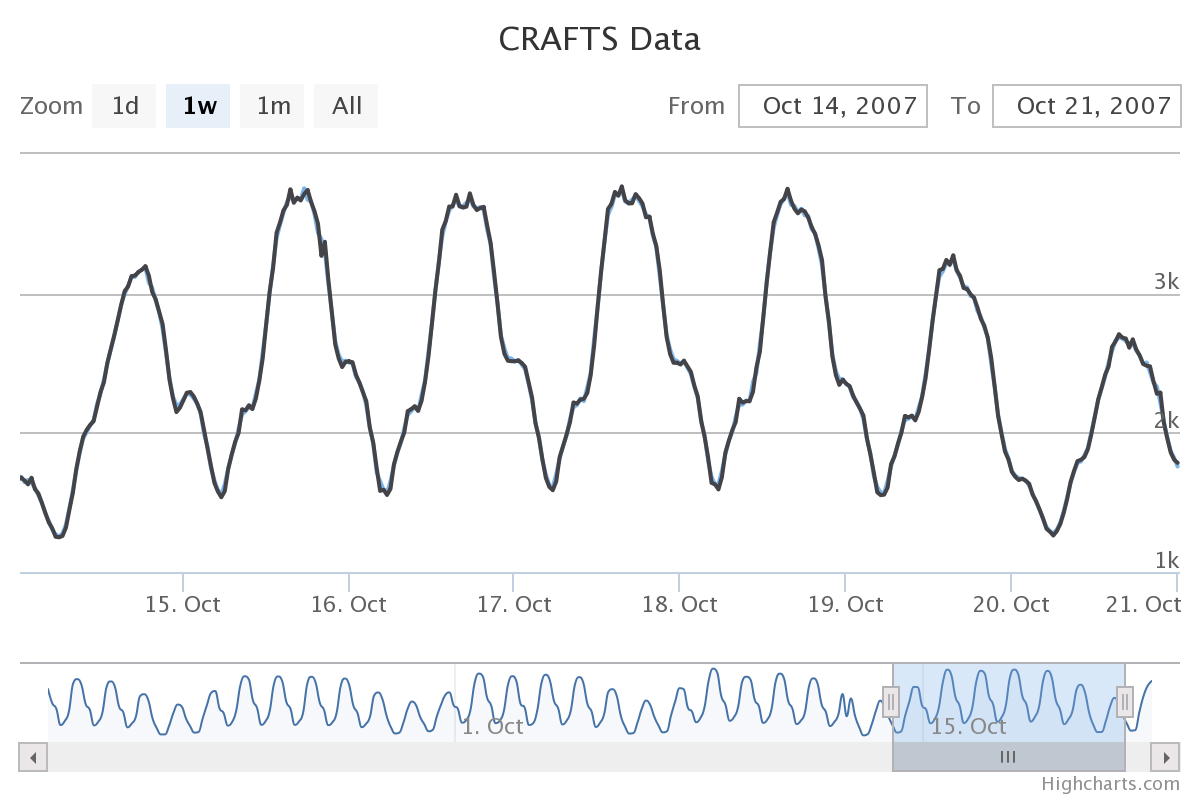
\includegraphics[width=\textwidth]{results/graphs/smoothing_training_outage.png}
\caption{Exponential smoothing prediction results for the training outage workload}
\label{fig:smoothing_to}
\end{figure}

\begin{table}[H]
\centering
\begin{tabular}{| l | l | l | l | l |}
\hline
Type & \multicolumn{2}{c |}{Regular} & \multicolumn{2}{c |}{Anomalous} \\ \hline
 & RMSD & Percent & RMSD & Percent \\ \hline
Under & 165 & 53.0\% & 1216 & 81.8\% \\ \hline
Over & 159 & 47.0\% & 3068 & 18.2\% \\ \hline
Total & 162 & & 1709 & \\ \hline
\end{tabular}
\caption{Exponential smoothing predictor results for the horizon outage workload}
\end{table}

\begin{figure}[H]
\centering
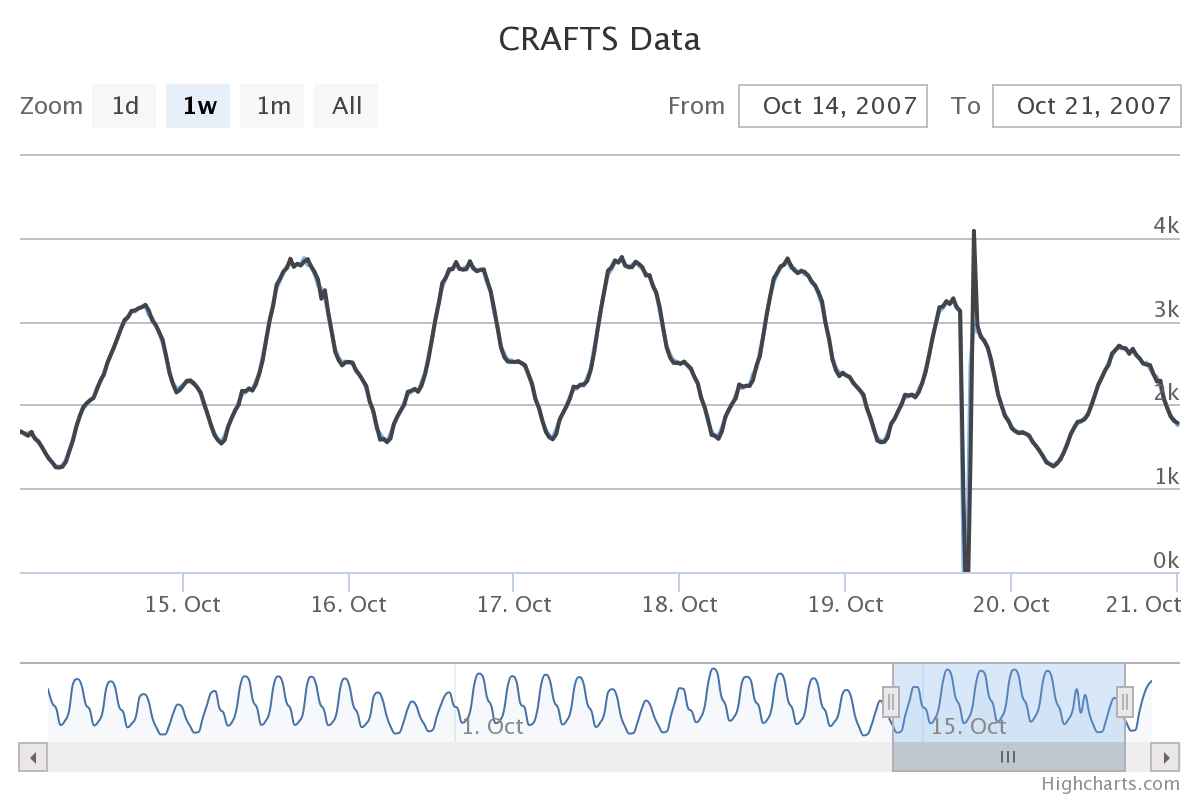
\includegraphics[width=\textwidth]{results/graphs/smoothing_horizon_outage.png}
\caption{Exponential smoothing prediction results for the horizon outage workload}
\label{fig:smoothing_ho}
\end{figure}

\begin{table}[H]
\centering
\begin{tabular}{| l | l | l | l | l |}
\hline
Type & \multicolumn{2}{c |}{Regular} & \multicolumn{2}{c |}{Anomalous} \\ \hline
 & RMSD & Percent & RMSD & Percent \\ \hline
Under & 42 & 53.2\% & 0 & 0.0\% \\ \hline
Over & 48 & 46.8\% & 16 & 100.0\% \\ \hline
Total & 45 & & 16 & \\ \hline
\end{tabular}
\caption{Exponential smoothing predictor results for the training spike workload}
\end{table}

\begin{figure}[H]
\centering
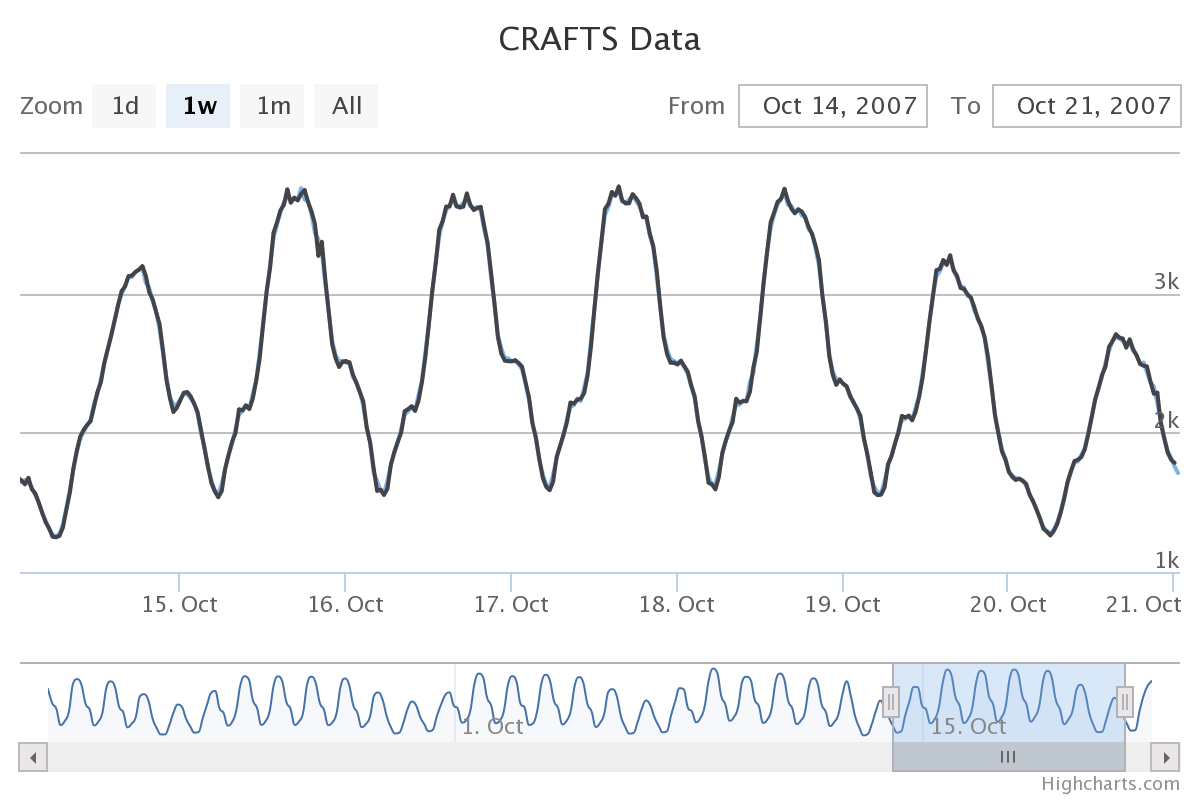
\includegraphics[width=\textwidth]{results/graphs/smoothing_training_spike.png}
\caption{Exponential smoothing prediction results for the training spike workload}
\label{fig:smoothing_ts}
\end{figure}

\begin{table}[H]
\centering
\begin{tabular}{| l | l | l | l | l |}
\hline
Type & \multicolumn{2}{c |}{Regular} & \multicolumn{2}{c |}{Anomalous} \\ \hline
 & RMSD & Percent & RMSD & Percent \\ \hline
Under & 129 & 53.2\% & 3036 & 100.0\% \\ \hline
Over & 277 & 46.8\% & 0 & 0.0\% \\ \hline
Total & 212 & & 3036 & \\ \hline
\end{tabular}
\caption{Exponential smoothing predictor results for the horizon spike workload}
\end{table}

\begin{figure}[H]
\centering
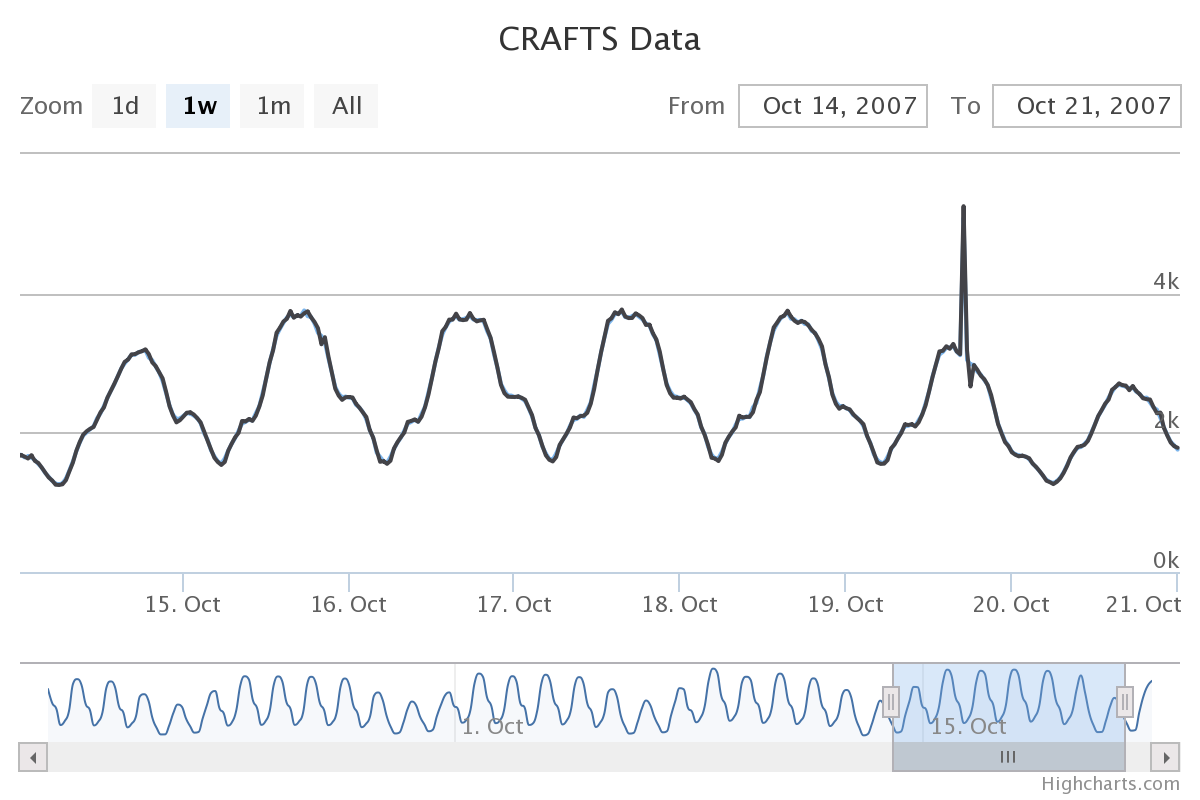
\includegraphics[width=\textwidth]{results/graphs/smoothing_horizon_spike.png}
\caption{Exponential smoothing prediction results for the horizon spike workload}
\label{fig:smoothing_hs}
\end{figure}